\documentclass[10pt,conference,compsocconf]{IEEEtran}

\usepackage{hyperref}
\usepackage{graphicx}	% For figure environment


\begin{document}
\title{Machine Learning -- Project 1}

\author{
  Pierre Fouche, Matthias Leroy and Alexandre Poussard\\
  \textit{MSc Data Science -- EPFL, Switzerland}
}

\maketitle

\begin{abstract}
  The aim of this paper is to make classification of particles over results' experiments. Thus, given a set of features that describe the decay signature of a collision event, we tried to predict if this event was a Higgs boson signal or some background information. We will expose the different machine learning algorithms we tried and the evaluations we made that finally led us to the ridge regression.
\end{abstract}

\section{Features Analysis and Data Preparation}

The training set is composed of $250 000$ samples of each $30$ features representing $30$ experimental measurements. During our dataset exploratory analysis, we noticed that the $23^{rd}$ feature (\textit{PRI.jet.num}) is discrete and categorical with values in the set $\{0,1,2,3\}$ which is different from all the other features. 

Moreover, the documentation of the contest (~\ref{sec:ref}) explained the dependence between the $23^{rd}$ column and all the other ones (some ones are not defined ($-999$) according to the value of \textit{PRI.jet.num}. That is why, we divided our data in three different sets according to the \textit{PRI.jet.num} values ($2$ and $3$ have the same features dependence, therefore we combined them). Thus, we could drop uninteresting features for each sets, that could allowed us to optimize the training. However, despite this first cleaning, we still had non-defined values ($-999$) in the first feature (\textit{DER.mass.MMC}). Thus, we decided to split again our three sets into $2$ smaller ones which contains defined or non-defined values in \textit{DER.mass.MMC} feature (and we drop this column for the non-defined ones).

Finally, we obtain six datasets depending on textit{PRI.jet.num} and \textit{DER.mass.MMC} with only defined values. This allows us to have two benefits for the computations: smaller training datasets and more precise one.

From now, we standardized each dataset and focused on polynomial basis. Thus, for each subset, we have at the beginning $N$ rows and $D$ features. For the polynomial basis, whose goal is to add new features for better training, we have a subset with still $N$ rows but $D\times d$ ($d$ = max degree). This degree is defined thanks to the cross-validation according to the model we use (more explained in next section). Instead of trying to find a different degree for each training dataset we could have chosen a common one big enough to satisfied each set. We would gain in test rapidity but with the risk to overfit the data.\\ 

Then, we realise that could added still more features in order to improve our prediction. However, features processing is more detailed in the last part of this report since we first implemented our models and then we tried to improve them thanks to features engineering.

\begin{table*}[htbp]
  \centering
  \begin{tabular}[c]{|c||c|c|c|c|c|c|c|c|}
    \hline
    Dataset&Loss&Lambda&Degree&Combination&Square&Cubic root&Absolute value&Square root \\
    \hline
    \hline
    jet0nm&0.4075&0.00908&2&False&False&True&True&True\\
    jet0wm&0.7313&$3.73\times10^{-7}$&3&True&False&True&False&True\\
    jet1nm&0.509&0.0177&2&False&False&True&True&True\\
    jet1wm&0.755&0.00069&4&True&False&True&True&True\\
    jet2nm&0.538&0.021&2&False&False&False&True&True\\
    jet2wm&0.7&0.0071&3&True&True&True&True&True\\
    \hline
  \end{tabular}
  \caption{Hyperparameters and features combinations for ridge regression using normal equations.}
  \label{tab:table1}
\end{table*}

\section{Models and Methods}
\label{sec:structure-paper}

In order to make our predictions, we tested $6$ different machine learning methods and tried to improve according to the results/validation evaluations we got. For a best model evaluation, we implemented a 5-fold cross-validation because we got validation sets of $50 000$ samples which is equivalent to a $20\%-80\%$ split of test and training data). 

We first tried a linear regression using a gradient descent. Our first questioning was to find a correct learning rate $\gamma$ in order to converge to the best parameters $\mathbf{w^*}$ for the minimum cost function that we could possibly find with this optimization algorithm. After testing different values for $\gamma$ it was finally possible to make our first prediction. 

This was very encouraging but we wanted to test other algorithms before started to optimize one. Thus, we implemented a stochastic gradient descent. We had to use a standard mini-batch-size-1. We did the same work, and tried to optimize the step-size. However, whatever its value was, we did not succeed to find a smaller loss that the one we got with the batch gradient descent. The only benefit of this method was the computational cost, in fact the convergence's speed was a little bit faster. 

However, at this step of the challenge, we were more concerned about efficiency and precision rather than complexity as long as our computer succeeded to get a result. Moreover, we could have tried mini-batch SGD and found a trade-off between speed and loss but we decided to find the optimum $\mathbf{w^*}$ parameters with least squares regression using normal equations. 

Actually, the solution is obtained explicitly by solving these normal equations and thus, optimize what we tried to do with gradient descents models. We got indeed better predictions using Least Square and we got a categorization accuracy of $0.80835$ on Kaggle. 

From this result, we tried to improve it with extended features vectors. Indeed, we added a polynomial basis in order to increase the representational power of the linear model. That's why we ran our cross-validation in order to determine the degree $M$ that minimize our validation error for each of our $6$ training sets. We improved our prediction with a $0.80929$ score. However, we noticed that the error for the training sets and the validation sets occasionally digressed a little for the best degrees. Thus, it could be resulting of an over-fitting problem. Therefore, in order to reduce our variance we tried to regularize our linear model by using ridge regression using normal equations. In fact, most of the work was to determine the hyper-parameters, since for this model we have to find a $\lambda$ parameter that best regularize our model by penalize complex ones for every polynomial basis we wanted to test. 

Therefore, after running our 5-fold cross-validation we find a set of 6 $degre, \lambda$ couples for each dataset, that minimize the losses. Finally, we got a better prevision than with the Least Square model, we obtained $0.83745$ on Kaggle. Surprisingly, the $lambdas$ that gave us the best results were a bit small, thus, Least Square model was not over-fitting that much as we can see in Figure \ref{fig:figure1}.
Then, we implemented the logistic regression with gradient descent. We had good hope for this model because it is supposed to be optimized for classification problems. However, after training our data and find our learning rate $\gamma$ (for the gradient descent) and the degrees of our polynomial basis we were not able to reduce the loss compared to the ridge regression. In fact, we got a prediction score of $0.83450$ on Kaggle, which was close but not good enough.
Finally, we did not succeed to implement the regularized logistic regression. Our cross validation never converge and we were not able to find our best hyper-parameters for this models.

\begin{figure}[tbp]
  \centering
  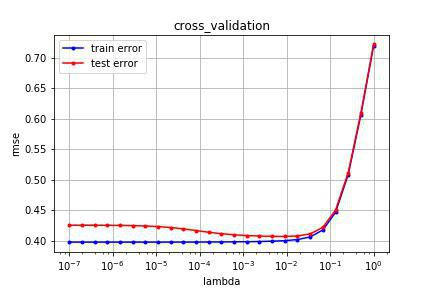
\includegraphics[width=\columnwidth]{cross-validation}
  \caption{5-fold cross-validation for ridge regression in order to find the best hyperparameter $\lambda$.}
  \vspace{-3mm}
  \label{fig:figure1}
\end{figure}

\section{Improving Prediction}

After, we found our best prediction, we asked ourself how we could continue to improve it. In fact, at the beginning of the challenge we tried models we have implemented directly on the 30 features dataset we downloaded and the polynomial basis. Without thinking about features engineering. It ended up with a very high bias over our estimation. In fact, it was not bother us to much when we start because the training and validation errors were very close when we ran the cross validation but, the error itself was not small enough for our prediction goal. That is why, we decided to add more features by modifying and combining existing ones depending on our training set. In fact, features engineering increases considerably our classification precision, but in return our training model needed more memory and took a longer processing time. Thus, we try different methods in order to find the best trade-off for each training set. 

First of all we compute the cross term matrix of our $D$ original features (the one to one product for each column) and get $C = \frac{D\times(D-1)}{2}$ new features. We also add the square, square root, cubic root and absolute value of these combinations. Thus, if we apply each of these new features to one of our training set, it is finally composed of $N$ samples and $D\times d + C\times5$ features. However, we didn't add all of these features to all of our training set but evaluated the importance of each thanks to our cross validation test and populated our set according to the losses we get.

Thus, we can see on the Table~\ref{tab:table1} the losses we got with the parameters and the combinations we used.

\section{Conclusion}

Finally, after trying different learning algorithm we achieved to find a prediction with a Kaggle score of $0.83912$ using the ridge regression with normal equation. In fact, we mainly increase our performances by improving and working on the features of the dataset. However, we think that could made even better with a regularized logistic with well tuned hyperparameters. Finally, it will be interesting to see what will be the effect of the more complex models we are going for this classification.

\section{Reference} \label{sec:ref}

\url{https://higgsml.lal.in2p3.fr/files/2014/04/documentation_v1.8.pdf}

\end{document}
